\documentclass{beamer}
\mode<presentation>
\usepackage{tikz}
\usepackage{multimedia}
\setbeamertemplate{caption}{\insertcaption}
\renewcommand{\thefootnote}{\fnsymbol{footnote}}
% \usepackage{pdfpcnotes}
\usetikzlibrary{shapes.geometric,positioning,math,lindenmayersystems}
\title{Understanding Teacher Needs for Starting and Running a Maths Circle}
\author[dishajk]{Maths Circle India Team}
\institute{International Centre for Theoretical Sciences - TIFR, Bangalore}
\date[SJU]{10 October 2025}
\begin{document}
\begin{frame}
    \titlepage
\end{frame}
\begin{frame}
    \frametitle{Outline}
    \tableofcontents[pausesections]
    \end{frame}
\section{What are Maths Circles?}
\begin{frame}
  \frametitle{What are Maths Circles?}
  Maths Circles are communities to nurture children's curiosity and talent in mathematics. They began as after-school programs in Soviet Union, where school teachers guided students to do problems outside their textbooks. They have since spread worldwide in many different forms.
\end{frame}
\section{ICTS experience}
\begin{frame}
  \frametitle{ICTS Experience}
  \begin{columns}[c]
    \begin{column}{0.45\textwidth}
      \begin{block}{ICTS-RRI Maths Circle}
        \begin{itemize}
          \item Meeting on 2nd and 4th Saturdays of every month at \alert{RRI, Mekhri Circle}.
          \item In collaboration with Raman Research Institute (RRI).
        \end{itemize}
      \end{block}
    \end{column}
    \begin{column}{0.45\textwidth}
      \begin{block}{Maths Circle India}
        \begin{itemize}
          \item Meeting on 1st and 3rd or 2nd and 4th Fridays over \alert{Zoom}.
          \item In collaboration with a network of institutions and people across India.
        \end{itemize}
      \end{block}
    \end{column}
  \end{columns}
\end{frame}
\subsection{Method}
\begin{frame}
  \frametitle{How we do it?}
  \begin{center}
  \movie[width=0.8\linewidth,height=0.6\linewidth,poster,autostart]
  {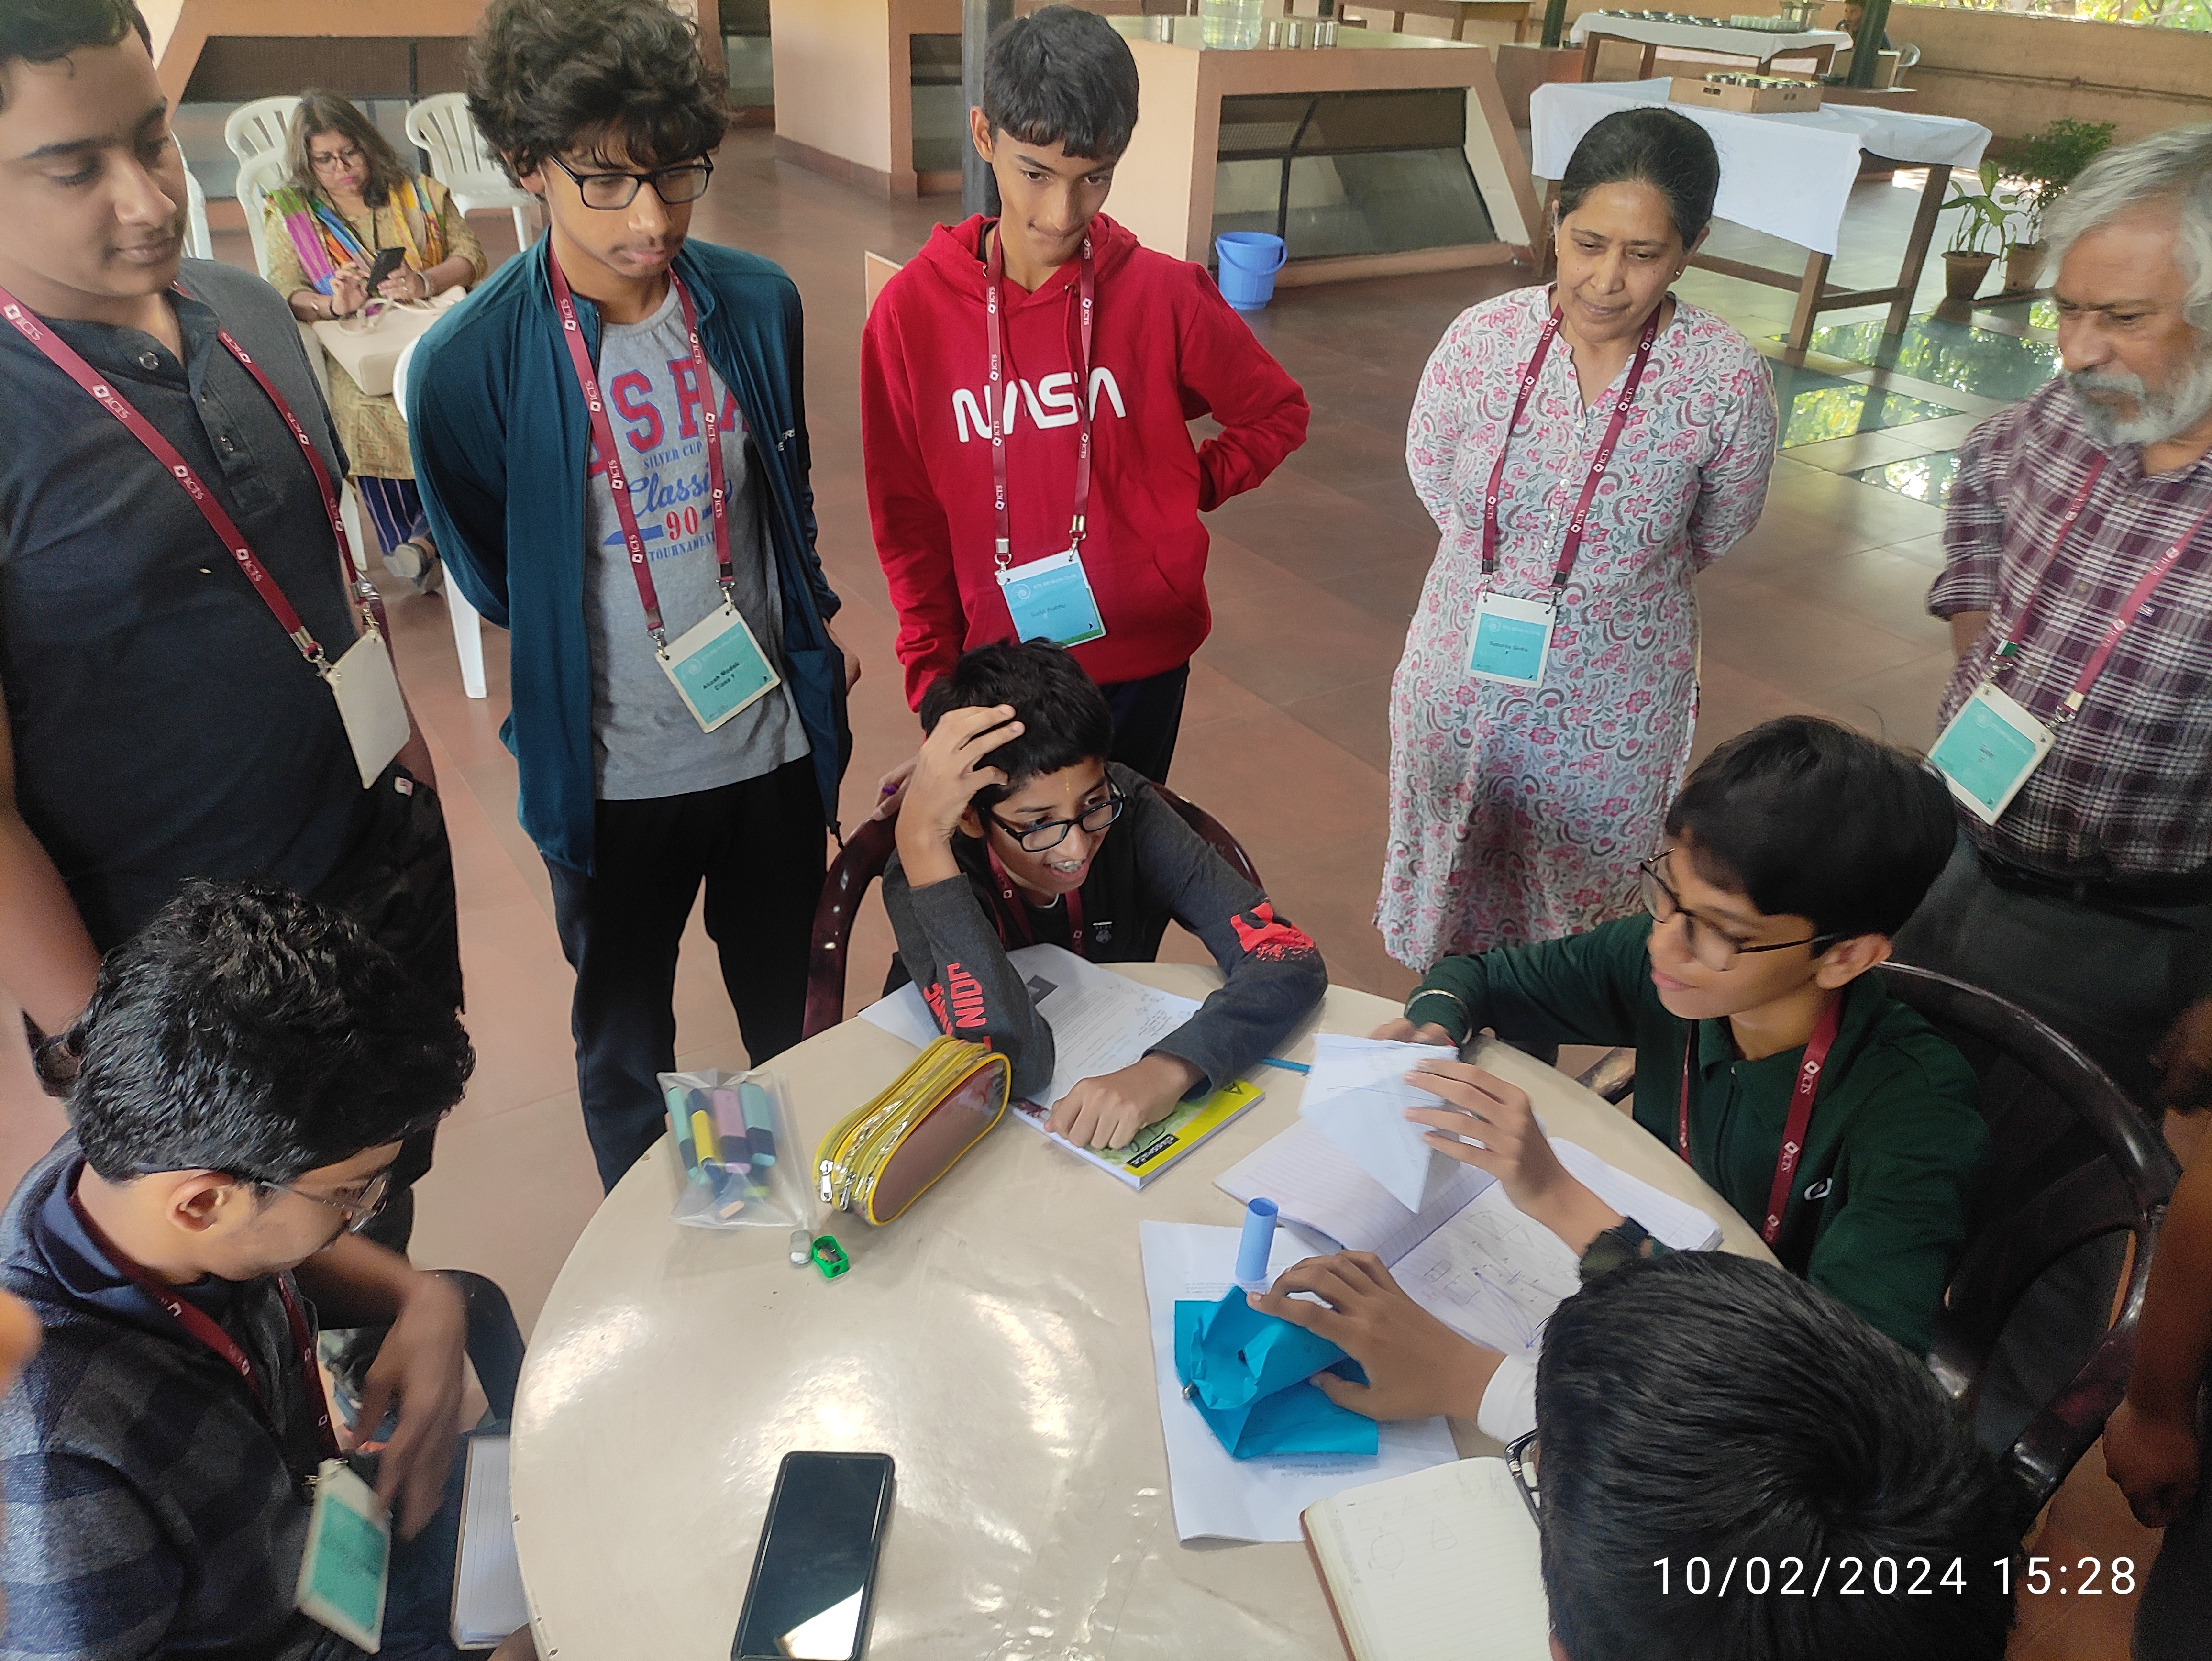
\includegraphics[width=0.5\linewidth]{ICTS-RRI-1.jpg}}{maths-circle.mp4}
  \end{center}
    % \movie[externalviewer]{\includegraphics[width=0.8\linewidth]{poster.png}}{maths-circle.mp4}
  % \hyperlinkmovie[]{}{/home/dishajk/Documents/Animate-Maths/media/videos/mathsCircle/2160p60/mathsCircle.mp4}

\end{frame}
\subsection{Other examples}
\begin{frame}
\frametitle{Other Maths Circles}
\animate<1-3>
\begin{figure}
  \only<1-3>{\caption{RAM Maths Circles}}  
  \only<1>{\includegraphics[width=0.6\linewidth]{RAM-1.png}\footnote{Image source: \url{raisingamathematician.com}}}
  \only<2>{\includegraphics[width=0.6\linewidth]{RAM-2.png}\footnote{Image source: \url{raisingamathematician.com}}}
  \only<3>{\includegraphics[width=0.6\linewidth]{RAM-3.png}\footnote{Image source: \url{raisingamathematician.com}}}
  \only<4>{\caption{Palakkad Maths Circle - IIT Palakkad}}
  \only<4>{\includegraphics[width=0.6\linewidth]{palakkad.jpg}\footnote{Image source: \url{mathcircle.iitpkd.ac.in}}}
  \only<5-6>{\caption{IISER Bhopal}}
  \only<5>{\includegraphics[width=0.6\linewidth]{bhopal-1.jpeg}\footnote{Image source: Ajit Bhand}}
  \only<6>{\includegraphics[width=0.6\linewidth]{bhopal-2.jpeg}\footnote{Image source: Ajit Bhand}}
\end{figure}
\end{frame}
\section{Need and Gaps}
\begin{frame}
  \frametitle{Needs and Gaps}
\end{frame}
\section{AMA}
\end{document}